\documentclass{exam}
\usepackage[utf8]{inputenc}
\usepackage{lmodern}
\usepackage{microtype}

% \usepackage[parfill]{parskip}
\usepackage[dvipsnames]{xcolor}
\usepackage{amsmath}
\usepackage{amsfonts}
\usepackage{amsthm}
\usepackage{siunitx}
\DeclareSIUnit\year{yr}
\DeclareSIUnit\foot{ft}
\DeclareSIUnit\litre{\liter}

\usepackage{skull}

\usepackage{pgfplots}
\usepgfplotslibrary{polar}
\pgfplotsset{compat=1.11}
\usepackage{graphicx}
\usepackage{sidecap}
\sidecaptionvpos{figure}{c}
\usepackage{float}
\usepackage{gensymb}
\usepackage{tkz-euclide}
\usetkzobj{all}
\usepackage{commath}
\usepackage{hyperref}
\usepackage{enumitem}
\usepackage{wasysym}
\usepackage{multicol}
\usepackage{mathtools}
\usepackage{tcolorbox}
\usepackage{tabularx}
\usepackage[version=4]{mhchem}
\usepackage{changepage}
\usepackage{listings}
\lstset{basicstyle=\ttfamily\linespread{0.8}\small}

\renewcommand*{\thefootnote}{\fnsymbol{footnote}}

\newtheorem*{thm}{Theorem}
\newtheorem*{iden}{Identity}
\newtheorem*{lemma}{Lemma}
\newtheorem{obs}{Observation}
\theoremstyle{definition}
\newtheorem*{defn}{Definition}
\newtheorem*{ex}{Example}
\newtheorem{con}{Construction}
\newtheorem*{alg}{Algorithm}

\newtheoremstyle{break}
  {\topsep}{\topsep}%
  {\itshape}{}%
  {\bfseries}{}%
  {\newline}{}%
\theoremstyle{break}
\newtheorem*{bthm}{Theorem}

% russian integral
\usepackage{scalerel}
\DeclareMathOperator*{\rint}{\scalerel*{\rotatebox{17}{$\!\int\!$}}{\int}}

% \DeclareMathOperator*{\rint}{\int}

\pgfplotsset{vasymptote/.style={
    before end axis/.append code={
        \draw[densely dashed] ({rel axis cs:0,0} -| {axis cs:#1,0})
        -- ({rel axis cs:0,1} -| {axis cs:#1,0});
    }
}}

% \pointsinrightmargin
\boxedpoints
\pointname{}

\newcommand{\questioA}{\question[\texttt{\textbf{\color{Cerulean} A}}]}
\newcommand{\questioM}{\question[\texttt{\textbf{\color{PineGreen} M}}]}
\newcommand{\questioE}{\question[\texttt{\textbf{\color{WildStrawberry} E}}]}
\newcommand{\questioS}{\question[\texttt{\textbf{\color{Goldenrod} S}}]}
\newcommand{\questioO}{\question[\texttt{\textbf{\color{BurntOrange} O}}]}

\newcommand{\parA}{\part[\texttt{\textbf{\color{Cerulean} A}}]}
\newcommand{\parM}{\part[\texttt{\textbf{\color{PineGreen} M}}]}
\newcommand{\parE}{\part[\texttt{\textbf{\color{WildStrawberry} E}}]}
\newcommand{\parS}{\part[\texttt{\textbf{\color{Goldenrod} S}}]}
\newcommand{\parO}{\part[\texttt{\textbf{\color{BurntOrange} O}}]}

\newcommand{\subparA}{\subpart[\texttt{\textbf{\color{Cerulean} A}}]}
\newcommand{\subparM}{\subpart[\texttt{\textbf{\color{PineGreen} M}}]}
\newcommand{\subparE}{\subpart[\texttt{\textbf{\color{WildStrawberry} E}}]}
\newcommand{\subparS}{\subpart[\texttt{\textbf{\color{Goldenrod} S}}]}
\newcommand{\subparO}{\subpart[\texttt{\textbf{\color{BurntOrange} O}}]}

\newcommand{\mainHeader}[2]{\section*{NCEA Level 2 Mathematics\\#1. #2}}
\newcommand{\mainHeaderHw}[2]{\section*{NCEA Level 2 Mathematics (Homework)\\#1. #2}}


\begin{document}

\mainHeader{18}{Graphs and Networks}
The final topic that we will look at is the theory of graphs. A graph is a set of points (called vertices) that are joined by
lines (edges), as in the following examples:

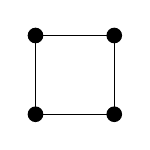
\begin{tikzpicture}
  \node[circle,fill,inner sep=2pt] at (0,0) {};
  \node[circle,fill,inner sep=2pt] at (0,1) {};
  \node[circle,fill,inner sep=2pt] at (1,1) {};
  \node[circle,fill,inner sep=2pt] at (1,0) {};
  \draw (0,0)--(0,1)--(1,1)--(1,0)--(0,0);
\end{tikzpicture}
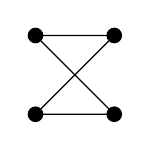
\begin{tikzpicture}
  \node[circle,fill,inner sep=2pt] at (0,0) {};
  \node[circle,fill,inner sep=2pt] at (0,1) {};
  \node[circle,fill,inner sep=2pt] at (1,1) {};
  \node[circle,fill,inner sep=2pt] at (1,0) {};
  \draw (0,0)--(1,1)--(0,1)--(1,0)--(0,0);
\end{tikzpicture}
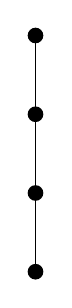
\begin{tikzpicture}
  \node[circle,fill,inner sep=2pt] at (0,0) {};
  \node[circle,fill,inner sep=2pt] at (0,1) {};
  \node[circle,fill,inner sep=2pt] at (0,2) {};
  \node[circle,fill,inner sep=2pt] at (0,3) {};
  \draw (0,0)--(0,1)--(0,2)--(0,3);
\end{tikzpicture}
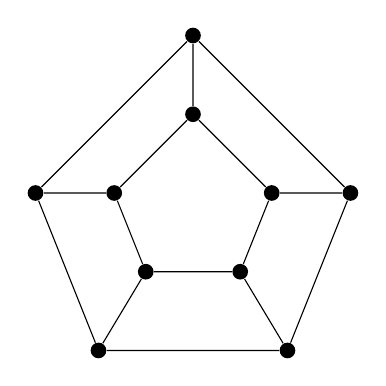
\begin{tikzpicture}
  \node[circle,fill,inner sep=2pt] (A) at (0,2) {};
  \node[circle,fill,inner sep=2pt] (B) at (0,1) {};
  \node[circle,fill,inner sep=2pt] (C) at (-2,0) {};
  \node[circle,fill,inner sep=2pt] (D) at (-1,0) {};
  \node[circle,fill,inner sep=2pt] (E) at (1,0) {};
  \node[circle,fill,inner sep=2pt] (F) at (2,0) {};
  \node[circle,fill,inner sep=2pt] (G) at (-0.6,-1) {};
  \node[circle,fill,inner sep=2pt] (H) at (0.6,-1) {};
  \node[circle,fill,inner sep=2pt] (I) at (-1.2,-2) {};
  \node[circle,fill,inner sep=2pt] (J) at (1.2,-2) {};
  \draw (A)--(B)--(D)--(C)--(D)--(G)--(I)--(G)--(H)--(J)--(H)--(E)--(F)--(E)--(B);
  \draw (A)--(C)--(I)--(J)--(F)--(A);
\end{tikzpicture}
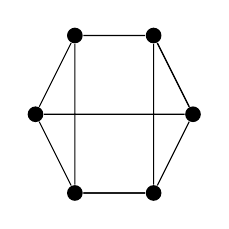
\begin{tikzpicture}
  \node[circle,fill,inner sep=2pt] (A) at (-0.5,1) {};
  \node[circle,fill,inner sep=2pt] (B) at (0.5,1) {};
  \node[circle,fill,inner sep=2pt] (C) at (-1,0) {};
  \node[circle,fill,inner sep=2pt] (D) at (1,0) {};
  \node[circle,fill,inner sep=2pt] (E) at (-0.5,-1) {};
  \node[circle,fill,inner sep=2pt] (F) at (0.5,-1) {};
  \draw (A)--(B)--(D)--(F)--(E)--(C)--(A);
  \draw (A)--(E)--(F)--(B)--(D)--(C);
\end{tikzpicture}
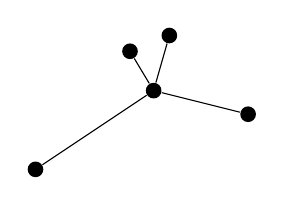
\begin{tikzpicture}
  \node[circle,fill,inner sep=2pt] (A) at (-0.3,0.5) {};
  \node[circle,fill,inner sep=2pt] (B) at (0.2,0.7) {};
  \node[circle,fill,inner sep=2pt] (C) at (-1.5,-1) {};
  \node[circle,fill,inner sep=2pt] (D) at (1.2,-0.3) {};
  \node[circle,fill,inner sep=2pt] (E) at (0,0) {};
  \draw (E)--(A)--(E)--(B)--(E)--(C)--(E)--(D);
\end{tikzpicture}
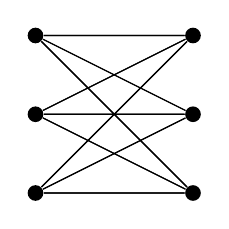
\begin{tikzpicture}
  \node[circle,fill,inner sep=2pt] (A) at (-1,1) {};
  \node[circle,fill,inner sep=2pt] (B) at (-1,0) {};
  \node[circle,fill,inner sep=2pt] (C) at (-1,-1) {};
  \node[circle,fill,inner sep=2pt] (D) at (1,1) {};
  \node[circle,fill,inner sep=2pt] (E) at (1,0) {};
  \node[circle,fill,inner sep=2pt] (F) at (1,-1) {};
  \draw (A)--(D)--(B)--(E)--(C)--(F)--(A);
  \draw (B)--(D)--(C)--(E)--(A)--(F)--(B);
  \draw (C)--(D)--(A)--(E)--(B)--(F)--(C);
\end{tikzpicture}

As we see at the left, the same graph can be drawn in different ways. The following nine drawings are all of the same graph, the
Petersen graph.

\begin{center}
  \includegraphics[width=0.5\textwidth]{petersen}
\end{center}

In this topic, we will only consider graphs that are \emph{finite}.

\begin{defn}\leavevmode
  \begin{itemize}
    \item Two vertices are \emph{adjacent} if there is an edge joining them.
    \item The \emph{order} of a vertex is the number of edges incident to it.
    \item If we label the vertices, then each edge can be identified by its endpoints: if an edge joins $ a $ and $ b $, we call the edge $ ab $.
    \item A \emph{path} on a graph between two vertices $ a $ and $ b $ is an ordered set of edges $ av_1, v_1 v_2, \dots, v_n b $ such
          that no edge is repeated.
    \item A \emph{cycle} is a path on the graph between $ a $ and itself.
    \item If every two vertices are connected by some path, then the graph is called \emph{connected}.
    \item If the graph has no cycles, it is called a \emph{tree}.
  \end{itemize}
\end{defn}

\subsection*{Traversibility}
Questions about paths and traversibility have been asked about graphs for hundreds of years. In 1736, Leonhard Euler solved the following problem:
\begin{center}
  \itshape
  The city of K\"onigsberg in Prussia was set on a river, and included two large islands connected by bridges as in the following diagram.
  \begin{center}
    \includegraphics[width=0.3\textwidth]{konigsberg}
  \end{center}
  Is it possible to walk a path in the city such that every bridge is crossed precisely once?
\end{center}
The answer, as we will see, is no. We begin by drawing a graph of the situation in order to eliminate all of the extraneous
details beyond the connectedness of the city.

\begin{center}
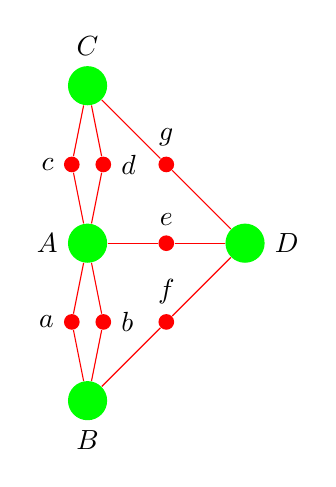
\begin{tikzpicture}
  \node[label=$C$,circle,fill,inner sep=5pt,color=green] (I1) at (0,2) {};
  \node[label=left:$A$,circle,fill,inner sep=5pt,color=green] (I2) at (0,0) {};
  \node[label=below:$B$,circle,fill,inner sep=5pt,color=green] (I3) at (0,-2) {};
  \node[label=right:$D$,circle,fill,inner sep=5pt,color=green] (I4) at (2,0) {};

  \node[label=right:$d$,circle,fill,inner sep=2pt,color=red] (B1) at (0.2,1) {};
  \node[label=left:$c$,circle,fill,inner sep=2pt,color=red] (B2) at (-0.2,1) {};
  \node[label=right:$b$,circle,fill,inner sep=2pt,color=red] (B3) at (0.2,-1) {};
  \node[label=left:$a$,circle,fill,inner sep=2pt,color=red] (B4) at (-0.2,-1) {};
  \node[label=$g$,circle,fill,inner sep=2pt,color=red] (B5) at (1,1) {};
  \node[label=$f$,circle,fill,inner sep=2pt,color=red] (B6) at (1,-1) {};
  \node[label=$e$,circle,fill,inner sep=2pt,color=red] (B7) at (1,0) {};

  \draw[color=red] (I1)--(B1)--(I2);
  \draw[color=red] (I1)--(B2)--(I2);
  \draw[color=red] (I2)--(B3)--(I3);
  \draw[color=red] (I2)--(B4)--(I3);
  \draw[color=red] (I1)--(B5)--(I4);
  \draw[color=red] (I2)--(B7)--(I4);
  \draw[color=red] (I3)--(B6)--(I4);
\end{tikzpicture}
\end{center}

A path that traverses every edge of a graph exactly once is called an Eulerian path (and an Eulerian path that is also
a cycle is called an Eulerian cycle).

\begin{thm}[Euler]
  A connected graph has an Eulerian path if and only if it has either zero or two vertices with odd order.
\end{thm}

We will prove the `only if' half here: that a graph has an Eulerian path only if it has zero or two vertices with odd order. The `only if'
part was proved by Carl Hierholzer in 1873.

\begin{proof}[Proof of necessity]
  Suppose a graph has an Eulerian path. Consider some vertex $ v $ that the path passes through. Then:
  \begin{enumerate}
    \item If the path does not have an endpoint on $ v $, then $ v $ has even order because every edge at the
          vertex is an edge of the path, and each time the path enters the vertex it leaves (so all the edges
          at $ v $ can be paired up).
    \item If the path has precisely one endpoint on $ v $, it has odd order, because all the edges but the
          endpoint edge can be paired up as in (1).
    \item If the path has two endpoints at $ v $, then $ v $ has even order, because we can pair the two endpoints together
          and then pair the other edges as in (1).
  \end{enumerate}
  Every vertex has odd order, except if a vertex falls under case (2). But this can happen at most twice (a path has only
  two endpoints), and if both endpoints are at different vertices then case (2) applies to both. Hence a graph with an
  Eulerian path has either zero or two vertices of odd order.
\end{proof}

Hence the K\"onigsberg challenge cannot be solved: there are more than two vertices of odd order.

\subsection*{Weighted graphs}
Graphs can be used to model situations in subjects including computer science, scheduling, linguistics, and biology. For example,
suppose some company has five distribution centres and wants to find an economical shipping pattern. Let's draw a graph with five
vertices and label the edges with the cost of sending a truck (in hundreds of dollars) between the two joined centres:
\begin{center}
  \includegraphics[width=0.3\textwidth]{graph1}
\end{center}
(If we label edges like this, the graph becomes a \emph{weighted graph}. The numbers are referred to as costs, weights, or distances.)

Suppose the company wants to send packages between every pair of distribution centrs, but does not want to pay to run all of the
routes graphed. What are the edges that we can safely delete? In practice, we want to find a minimum spanning tree for this graph:
a subgraph, without cycles, so that the total cost of the subgraph is a minimum. (Finding this graph would allow this company to
minimise expendiature while not losing any connections.) One algorithm to find the minimum spanning tree is the reverse-delete algorithm:
\begin{alg}[Reverse-delete]\leavevmode
  \begin{enumerate}
    \item List all of the edges in descending weight-order.
    \item Examine each edge in order, starting with the most expensive. If deleting this edge disconnects the graph, do not remove
          the edge; otherwise, remove the edge.
  \end{enumerate}
  The remaining graph is a minimum spanning tree.
\end{alg}
For example, in this case we obtain the following minimum spanning tree:
\begin{center}
  \includegraphics[width=0.3\textwidth]{graph2}
  \includegraphics[width=0.3\textwidth]{graph3}
\end{center}

On the other hand, suppose the company does not run all its routes constantly and instead wants to find the cheapest route for a particular
package from one centre to another, utilising any of the eight edges above. This can be done with Dijkstra's algorithm:
\begin{alg}[Dijkstra]\leavevmode
  Suppose we want to find the shortest path from some vertex $ a $ to some vertex $ b $. In fact, this algorithm will
  give us the shortest path from $ a $ to \emph{any} other vertex!

  Label vertex $ a $ with zero and every other vertex as $ \infty $; then set $ a $ as the current vertex, and:
  \begin{enumerate}
    \item Consider every unvisited vertex $ v $ directly adjacent to the current vertex, and update the label of $ v $ to the smallest value out of:
      \begin{itemize}
        \item Either the current value on $ v $, or
        \item The sum of the current value on the current vertex and the distance from the current vertex to $ v $.
      \end{itemize}
    \item If the vertex $ v $ has been relabeled by step (1), then mark with an arrow the edge joining the current vertex with $ v $ and unmark any
          other edges on $ v $ that have been marked in previous steps.
    \item Label the current vertex as visited.
    \item If every vertex is visited, then we halt; otherwise, set the current vertex to the vertex with minimal label and repeat from step (1).
  \end{enumerate}
  Each vertex $ v $ is now labeled with the minimum distance from $ a $ to $ v $, and the shortest path from $ a $ to $ v $ is marked by the arrows.
\end{alg}

\subsection*{Questions}
\begin{questions}
  \question Justify, with mathematical reasoning, the following statements.
    \begin{parts}
      \part A graph that is not connected has no Eulerian paths.
      \part If a graph has no vertices of odd order, all Eulerian paths are circuits; if there are two vertices with
            odd order, all Eulerian paths begin at one and end at the other.
      \part The sum of all the orders of all the vertices must be even.
    \end{parts}
  \question Consider the K\"onigsberg bridge graph.
    \begin{parts}
      \part Show that it is possible to exhibit a Eulerian path on the graph resulting from adding a single extra bridge.
      \part Show that, no matter where the bridge is placed, there will still be no Eulerian circuit.
    \end{parts}
  \question Suppose there are three houses on a flat plane (or plain), and each needs to be connected to water, gas, and electricity.
    \begin{parts}
      \part Show that this is impossible without two connections crossing, without using a third dimension or running a connection through a house.
      \part Show that, on a torus (a doughnut), it \emph{is} possible.
    \end{parts}
  \question Legend has it that an ancient Indian lord had five sons, and he allowed them to split his land up after his death between
            them, on the proviso that the land of each son must be in one piece, and must share a boundary with the land of all four
            other sons. Why is this funny?
  \clearpage
  \question Consider the following weighted graph $ G $.
            \begin{center}
              \includegraphics[width=0.3\textwidth]{graph4}
            \end{center}
    \begin{parts}
      \part Give an example of a graph with more than one minimal spanning tree.
      \part Show that $ G $ has precisely one minimal spanning tree.
      \part Find a vertex $ v $ of $ G $ such that the minimal spanning tree of the graph also gives the shortest paths from $ v $ to every other vertex.
    \end{parts}
  \question Find the cheapest shipping path between distribution centres 1 and 3 in the example of a weighted graph from above (reproduced here).
            \begin{center}
              \includegraphics[width=0.2\textwidth]{graph1}
            \end{center}
  \question Suppose that, in addition to weights on edges of a graph, we assign a direction: perhaps we are modelling the direction and velocity
            of some fluid flow. Consider the following directed graph:
            \begin{center}
              \includegraphics[width=0.3\textwidth]{digraph}
            \end{center}
    \begin{parts}
      \part Call a directed graph connected if we can give a directed path from every vertex $ a $ to every other
            vertex $ b $ (i.e. a path with arrows from $ a $ to $ b $). Explain why this directed graph is not connected.
      \part Find the shortest path from vertex 4 to every other vertex.
    \end{parts}
  \question A \textbf{Hamiltonian path} is a path on a graph such that every vertex appears on the path exactly once. If the two endpoints
            of the path are adjacent, then the path is called a \textbf{Hamiltonian cycle}. Find a Hamiltonian cycle on the dodecahedron graph:
            \begin{center}
              \includegraphics[width=0.2\textwidth]{dodec}
            \end{center}
            The existence of Hamiltonian paths on graphs is much more difficult than the existence of Eulerian paths. One recent result (from
            2005) is that a graph with $n$ vertices has a Hamiltonian path if, for every pair of non-adjacent vertices, the sum of their degrees
            and the distance between them is greater than $n$.
\end{questions}

\end{document}
